

\section{Computational models for brain simulation}

The coupled differential equations that define a compartmental model of a neuron
can be solved numerically, and can therefore be programmed in a high-level
programming language relatively simply. However, while programmatically solving
differential equations is straightforward in principle, the computational power
and provision of memory required makes simulating large networks of neurons
difficult to do in practice \autocite{trappenberg_fundamentals_2009}. Existing
simulation packages provide a foundation from which biological experiments can
be conducted, and aim to abstract away purely computational concerns. Some of
these packages that have different approaches to solving this are described in
more detail below.

\subsection{Representing time in neural simulations}

There are several approaches that can be taken with respect to both simulating
individual neuron activity, and more general network activity. On the level of
individual components of a simulated network, the two predominant choices are
between a clock driven model and an event driven model. In a clock driven model,
continuous time is split into discrete chunks, and it is the size of these
chunks that determine the accuracy of the differential equations that define
neuronal behaviour. Meanwhile, an event driven model is asynchronous in nature,
where events such as spikes or learning updates that propagate backwards will
trigger further updates across the network. The advantage of a clock driven
model is its flexibility in using any differential equation, however, more
complex neuron models require a smaller time step leading to large computation
times. An event driven model, by comparison, computes in real time and spikes
are therefore unaffected by rounding errors from discretization
\autocite{brette_simulation_2007}. It is also possible to simulate population
dynamics to describe the average activity of neuronal populations
\autocite{trappenberg_fundamentals_2009}, which is ideal for modelling neuronal
populations that are on the scale of actual nervous systems with modern
computational power. The downside to this, however, is that such generalised
models are not always faithful approximations of true network effects between
neurons.

\subsection{Available neural simulation and modelling software packages}

\subsubsection{VERTEX}
The Virtual Electrode Recording Tool for EXtracellular potentials (VERTEX) is a
simulator for large networks of neurons written in the MATLAB programming
language. More specifically, it aims to reproduce the measurements that are
produced by in-vivo recordings from patients fitted with multi-electrode
arrays. This is achieved by locating each neuron in 3D space, placing virtual
electrodes in the same space, and calculating the change in potential at each
stage of the simulation at each electrode. The neuron model used in VERTEX is
also more advanced than similar models described in this section in that the
local field potential (LFP) of the neuron is spatially realistic
\autocite{tomsett_virtual_2015}. A major advantage of this design is that it
becomes easy to map between general neuronal activity in a simulated model and
brain activity of, say, a real-world patient in a medical trial.

A 2019 update to VERTEX introduced a range of simulation features, the most
notable of which for the purposes of this project is Spike Time Dependent
Plasticity (STDP), which dynamically adapts the weighting of synapses based on
the observed causality of pre-synaptic spikes on post-synaptic spikes
\autocite{thornton_virtual_2019}. Details on how this may be implemented and
used are covered further in Chapter 3.

VERTEX itself is multithreaded, and makes use of the compute pooling feature in
MATLAB to separate groups of tasks into separate logical threads. This means
that, with a sufficiently large model, doubling the number of available workers
in the pool nearly halves the time taken to simulate, as shown in figure
\ref{VERTEXparallel} below.

\begin{figure}[h!]
    \centering
    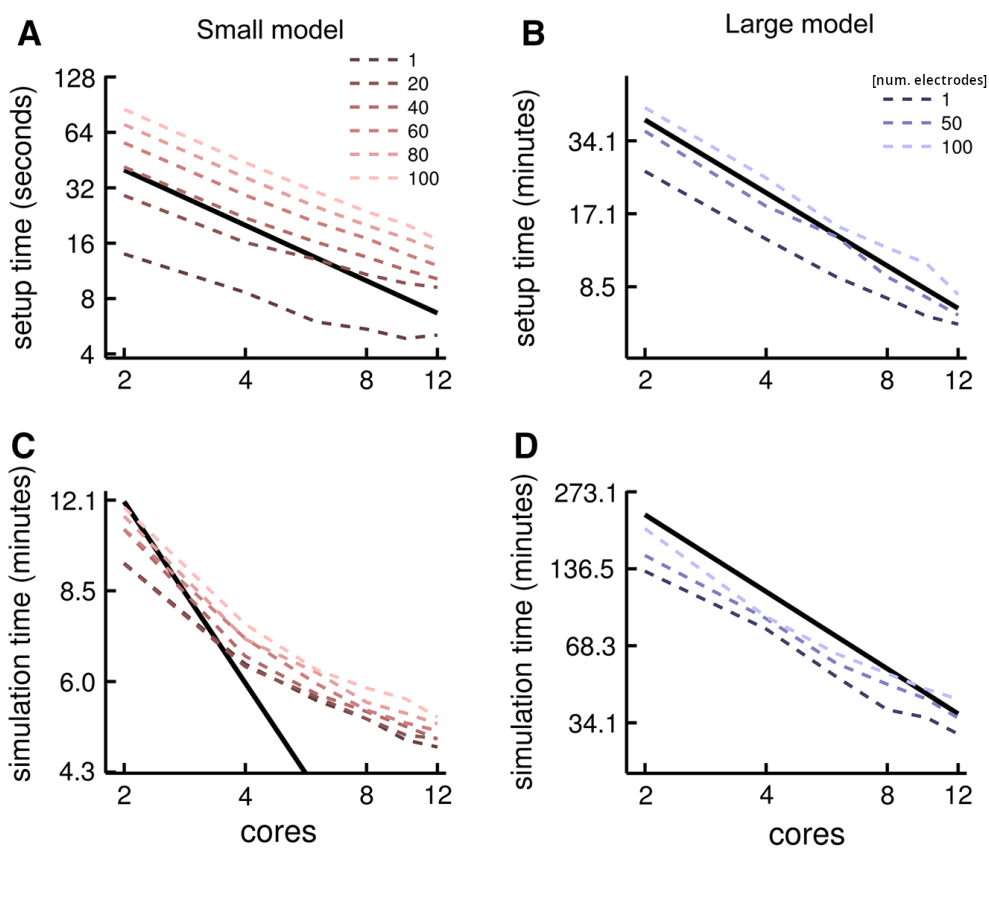
\includegraphics{figures/graphs/coresVERTEX.png}
    \DoubleCaption{Impact of parralel computation on
        simulation performance in VERTEX} {\small{\cite{tomsett_virtual_2015}}}
    \label{VERTEXparallel}
\end{figure}
\vspace{1ex}

\subsubsection{NEURON}

NEURON describes itself as ``a tool designed specifically for solving the
equations that describe nerve cells'' and provides a holistic environment for
developing and simulating models of individual neurons and neural networks. It
is particularly adept at modelling complex chemistry in neuron models, and can
be used when the field potential of a location very close to a neuron needs to
be accurately modelled \autocite{carnevale_neuron_2006}. This does, however,
mean that simulating large networks is computationally expensive, and more
complex models require correctly tuned parameters for each new feature which
increases the time setting up simulations.

Further simulation toolkits may be built atop NEURON, and one such example is
LFPy. LFPy is a Python tool using NEURON that aims to accurately provide
extracellular potential readings for single neuron models
\autocite{hagen_hybrid_2016}. It can also provide extracellular potential
readings for networks in the most recent versions \autocite{hagen_lfpy_2019},
however the caveat that NEURON based networks are limited in size by available
resources still holds.

\subsubsection{Brian}

"Brian" is another simulator for spiking neural networks, distributed as a
Python library. Brian offers a unique programming interface whereby the
differential equations that define a Neuron can be written in plain-text and are
interpreted at runtime. Provided the equation can be interpreted, this approach
makes computing mathematical models extremely simple, and is ideal for quickly
testing variations of a model \autocite{stimberg_brian_2019}. This is, however,
less useful for more complex relationships between neurons where the plain-text
mathematical syntax develops its own API on top of the Python API. Fortunately
users of the library may provide native Python functions to define the behaviour
of their neurons if desired \autocite{noauthor_functions_2020}. The complexity
of actual neurons in a Brian simulation is as complex as a programmer intends it
to be: Neurons can be placed in physical space if desired, but this is optional.
The time taken to simulate a network is largely dependant on the time complexity
of the user-defined equations that define the neurons.

\subsection{Similarities in existing software packages}

Each of the software packages described above is capable of doing simulating a
network of Neurons, but each has a distinct set of goals. Some, like Brian, are
intended as tools to study the spiking patterns and features of generic neural
networks, while VERTEX provides a more specialised tool that is optimised for
measuring the observed potential changes in a similar manner to capturing
experimental data. These differences are also seen in the API available to
developers
and the distribution methods that each package uses. VERTEX requires that the
user defines the parameters for Neuron grouping and placement while abstracting
away the exact definition of the Neuron behaviour, while NEURON and Brian are
very much focussed on the Neuron definition, and space placement and recording
mechanisms are functions largely left to the programmer to define.